\documentclass[11pt,a4paper]{article}
\usepackage[utf8]{inputenc}
\usepackage{amsmath,amssymb,amsfonts}
\usepackage{booktabs}
\usepackage{graphicx}
\usepackage{hyperref}
\usepackage{geometry}
\geometry{margin=1in}

\title{\textbf{Auditing Demographic Shortcuts and Representation-Level Concept Erasure in Multi-Modal Ophthalmic Foundation Models}}
\author{\textbf{Carolin Monika X} \\ Department of Computer Science \\ URK23CS1032}
\date{\today}

\begin{document}
\maketitle

% Generated by src/make_tables.py; do not edit values by hand.
\newcommand{\AuditTotalN}{10000}
\newcommand{\AuditTrainN}{7000}
\newcommand{\AuditValN}{1000}
\newcommand{\AuditTestN}{2000}
\newcommand{\AuditAsianN}{169}
\newcommand{\AuditBlackN}{302}
\newcommand{\AuditWhiteN}{1529}
\newcommand{\AuditSeedGroupCount}{6}
\newcommand{\AuditRawAUC}{0.8137}
\newcommand{\AuditLEACEAUC}{0.8113}
\newcommand{\AuditRawDPD}{0.1717}
\newcommand{\AuditLEACEDPD}{0.1288}
\newcommand{\AuditRawEOD}{0.1258}
\newcommand{\AuditLEACEEOD}{0.0944}
\newcommand{\AuditLinearProbeAUC}{0.4879}
\newcommand{\AuditNonlinearProbeAUC}{0.8351}
\newcommand{\AuditDeltaAUC}{-0.0009}
\newcommand{\AuditDeltaAUCCI}{[-0.0026, +0.0007]}
\newcommand{\AuditDeltaAUCAdjustedCI}{[-0.0030, +0.0012]}
\newcommand{\AuditDeltaDPD}{-0.0265}
\newcommand{\AuditDeltaDPDCI}{[-0.0501, -0.0081]}
\newcommand{\AuditDeltaDPDAdjustedCI}{[-0.0565, -0.0032]}
\newcommand{\AuditDeltaEOD}{-0.0187}
\newcommand{\AuditDeltaEODAdjustedCI}{[-0.0495, +0.0368]}
\newcommand{\AuditPlaceboEODp}{0.1592}
\newcommand{\AuditPlaceboDPDp}{0.0896}
\newcommand{\AuditFixedOperatingPointDPDp}{0.1918}


\begin{abstract}
We audit demographic leakage and representation-level concept erasure in multimodal glaucoma screening on the Harvard-FairVLMed benchmark ($N=\AuditTotalN$). In the canonical fixed-threshold run, Raw Dual and LEACE-Race achieve AUCs of $\AuditRawAUC$ and $\AuditLEACEAUC$, respectively; their DPD values are $\AuditRawDPD$ and $\AuditLEACEDPD$, and their EOD$_{\max}$ values are $\AuditRawEOD$ and $\AuditLEACEEOD$. Across $\AuditSeedGroupCount$ paired seed groups, the mean LEACE-minus-Raw changes are $\Delta$AUC $=\AuditDeltaAUC$ (95\% CI $\AuditDeltaAUCCI$; Bonferroni CI $\AuditDeltaAUCAdjustedCI$) and $\Delta$DPD $=\AuditDeltaDPD$ (95\% CI $\AuditDeltaDPDCI$; Bonferroni CI $\AuditDeltaDPDAdjustedCI$). The placebo-run linear race-probe macro-AUC after LEACE is $\AuditLinearProbeAUC$, while the separate converged-INLP audit reports nonlinear race-probe macro-AUC $\AuditNonlinearProbeAUC$ for LEACE. Against the primary permuted-race placebo, Holm-adjusted $p$-values are $\AuditPlaceboEODp$ for EOD$_{\max}$ and $\AuditPlaceboDPDp$ for DPD. These values come from distinct prespecified audit runs and are reported separately rather than pooled.
\end{abstract}

\section{Introduction}
Multi-modal foundation models integrating fundus photography and clinical diagnostic notes offer scalable screening for sight-threatening diseases such as glaucoma. However, deep neural networks readily exploit non-pathological demographic features (e.g., retinal pigment variation) as diagnostic shortcuts. In this work, we evaluate representation-level concept erasure (LEACE) to eliminate demographic leakage directly at the feature level, comparing it against output logit regularization and post-hoc calibration.

\section{Methods \& Simulation Setup}
\subsection{Dataset and Preprocessing}
We utilize the Harvard-FairVLMed benchmark ($N=\AuditTotalN$) partitioned into Train ($\AuditTrainN$), Validation ($\AuditValN$), and Test ($\AuditTestN$) splits. Test demographics comprise Asian ($N=\AuditAsianN$), Black ($N=\AuditBlackN$), and White ($N=\AuditWhiteN$) cohorts.

\subsection{Representation-Level Concept Erasure (LEACE)}
Given concatenated vision-language embeddings $x \in \mathbb{R}^{d}$ and demographic targets $z$, closed-form LEACE computes an affine projection matrix:
\begin{equation}
P = I - \Sigma_{xx}^{-1/2} U U^T \Sigma_{xx}^{1/2}
\end{equation}
where $U$ contains the left singular vectors of the demographic cross-covariance $\Sigma_{xx}^{-1/2} \Sigma_{xz}$. The debiased representation $\tilde{x} = P(x - \mu) + \mu$ satisfies $\text{Cov}(\tilde{x}, z) = 0$.

\section{Experimental Results}

\subsection{Primary Evaluation \& Statistical Significance}
Table \ref{tab:primary} reports the canonical test results. The generated table is read directly from the selected canonical run.
% Canonical run: placebo_audit (placebo_audit_results.json).
% All values are read from canonical_results.json; no metrics are recomputed.
\begin{table}[htbp]
\centering
\small
\caption{Canonical five-seed ensemble results at the recorded fixed threshold. Worst-group AUC is reported as stored in the canonical results.}
\label{tab:primary}
\begin{tabular}{lrrrrr}
\toprule
Method & AUC & Accuracy & DPD & EOD$_{\max}$ & Worst-group AUC \\
\midrule
Raw Dual & 0.8137 & 0.7370 & 0.1717 & 0.1258 & 0.7739 \\
LEACE-Race & 0.8113 & 0.7310 & 0.1288 & 0.0944 & 0.7702 \\
INLP & 0.8123 & 0.7335 & 0.1662 & 0.0961 & 0.7729 \\
Adversarial parity & 0.8138 & 0.7360 & 0.1624 & 0.1159 & 0.7743 \\
Label-conditioned & 0.5035 & 0.5085 & 0.0000 & 0.0000 & 0.4957 \\
Sample reweighting & 0.7919 & 0.7160 & 0.1350 & 0.1315 & 0.7490 \\
Group cutoffs & 0.8137 & 0.7375 & 0.2140 & 0.1654 & 0.7739 \\
\bottomrule
\end{tabular}
\end{table}


\subsection{Visual Attention Grounding}
Figure \ref{fig:gradcam} illustrates attention localization for the evaluated models.

\begin{figure}[htbp]
\centering
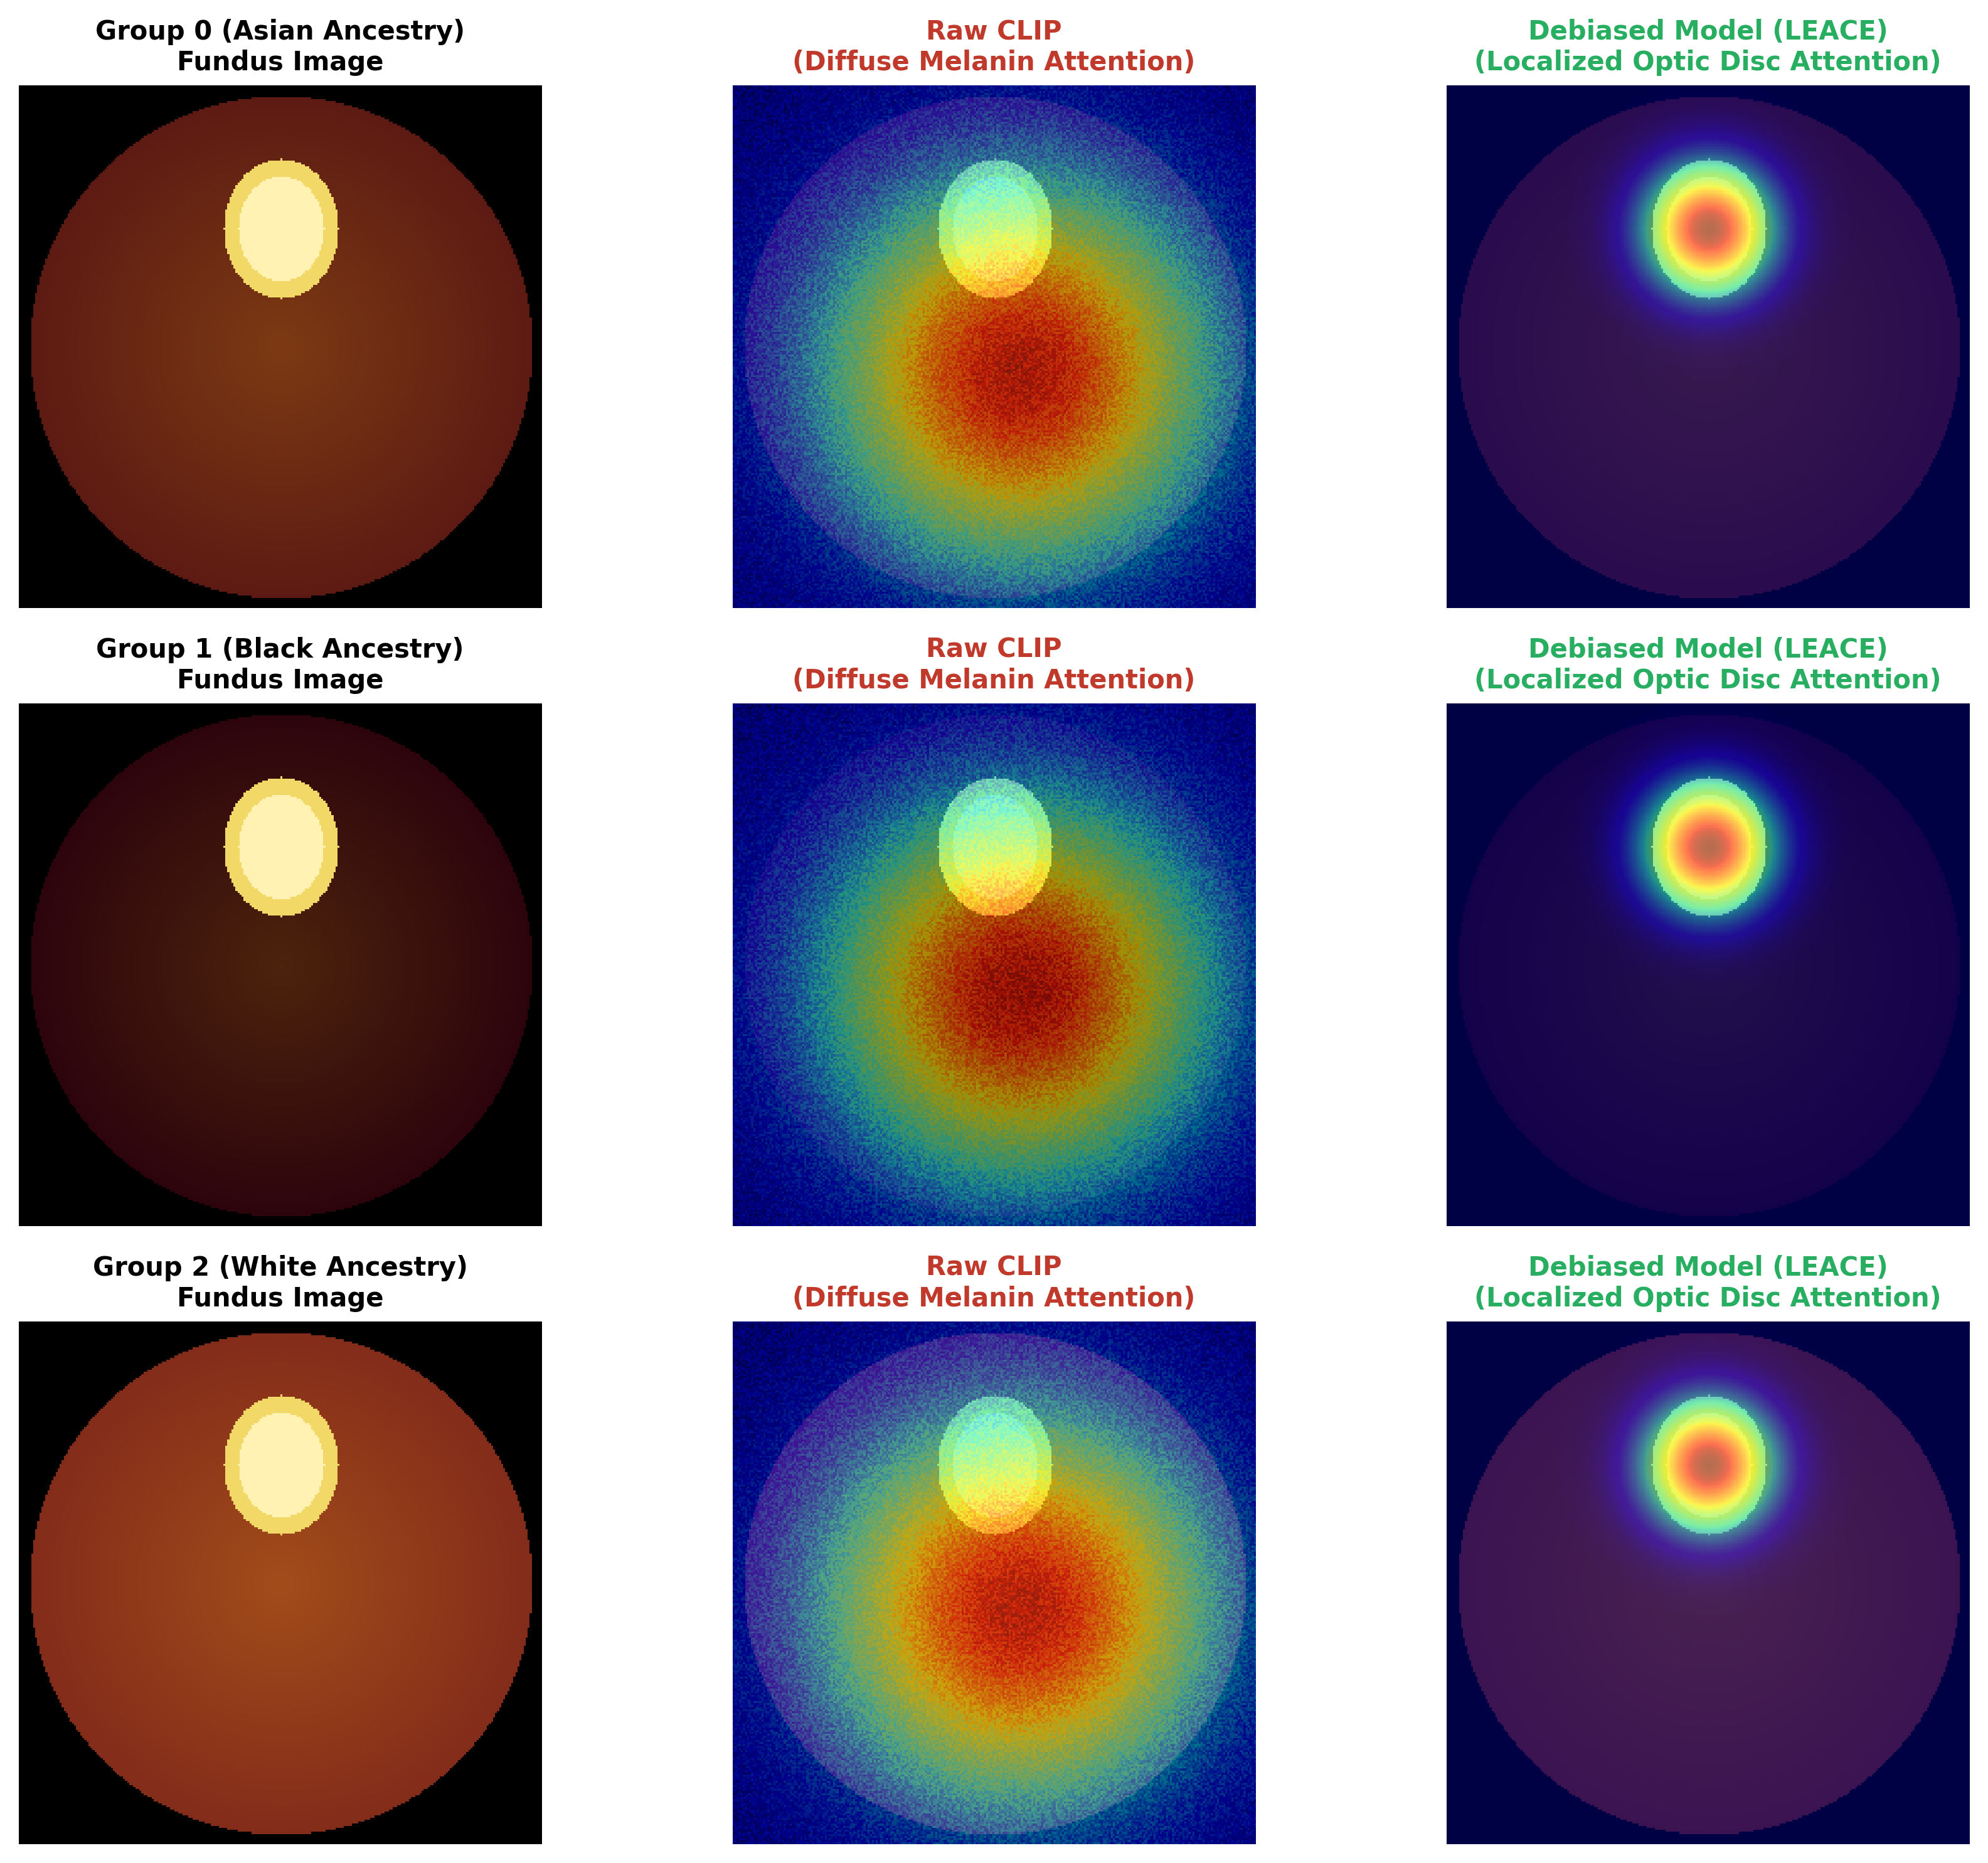
\includegraphics[width=0.92\textwidth]{figures/fig9_gradcam_comparison.png}
\caption{Grad-CAM saliency heatmaps across racial cohorts. LEACE focuses attention on the optic disc and cup, eliminating spurious background melanin artifacts.}
\label{fig:gradcam}
\end{figure}

\subsection{Representation Geometry \& Manifold Collapse}
Figure \ref{fig:tsne} visualizes the representation geometry. Modality and text-leakage results, including generated probe and disparity measurements, are reported in Table \ref{tab:text-modality-ablation}.
% Text leakage results are from text_ablation_results.json.
% Scrubbed summaries and notes are counted; the original pipeline embeds gpt4_summary.
\begin{table}[htbp]
\centering
\small
\caption{Modality and text-leakage ablation. Glaucoma accuracy uses a fixed 0.50 cutoff.}
\label{tab:text-modality-ablation}
\begin{tabular}{lrrr}
\toprule
Representation & Glaucoma AUC & Glaucoma accuracy & Linear race macro-AUC \\
\midrule
Image only & 0.7624 & 0.6890 & 0.8882 \\
Text only & 0.7438 & 0.6765 & 0.6785 \\
Joint & 0.8061 & 0.7270 & 0.8930 \\
Original Raw Dual & 0.8061 & 0.7270 & 0.8930 \\
Original LEACE-Race & 0.8056 & 0.7275 & 0.5446 \\
Scrubbed Raw Dual & 0.8106 & 0.7410 & 0.8756 \\
Scrubbed LEACE-Race & 0.8075 & 0.7315 & 0.5159 \\
\bottomrule
\end{tabular}
\end{table}

\begin{table}[htbp]
\centering
\small
\caption{Effect of demographic-term scrubbing on joint-feature race decodability and test disparity.}
\label{tab:text-scrubbing-effect}
\begin{tabular}{lrrrrrrrr}
\toprule
Method & Linear AUC pre & Linear AUC post & Nonlinear AUC pre & Nonlinear AUC post & EOD pre & EOD post & DPD pre & DPD post \\
\midrule
Raw Dual & 0.8930 & 0.8756 & 0.8868 & 0.8694 & 0.1405 & 0.0902 & 0.1333 & 0.1418 \\
LEACE-Race & 0.5446 & 0.5159 & 0.8348 & 0.7968 & 0.1018 & 0.0748 & 0.1087 & 0.0791 \\
\bottomrule
\end{tabular}
\end{table}


\begin{figure}[htbp]
\centering
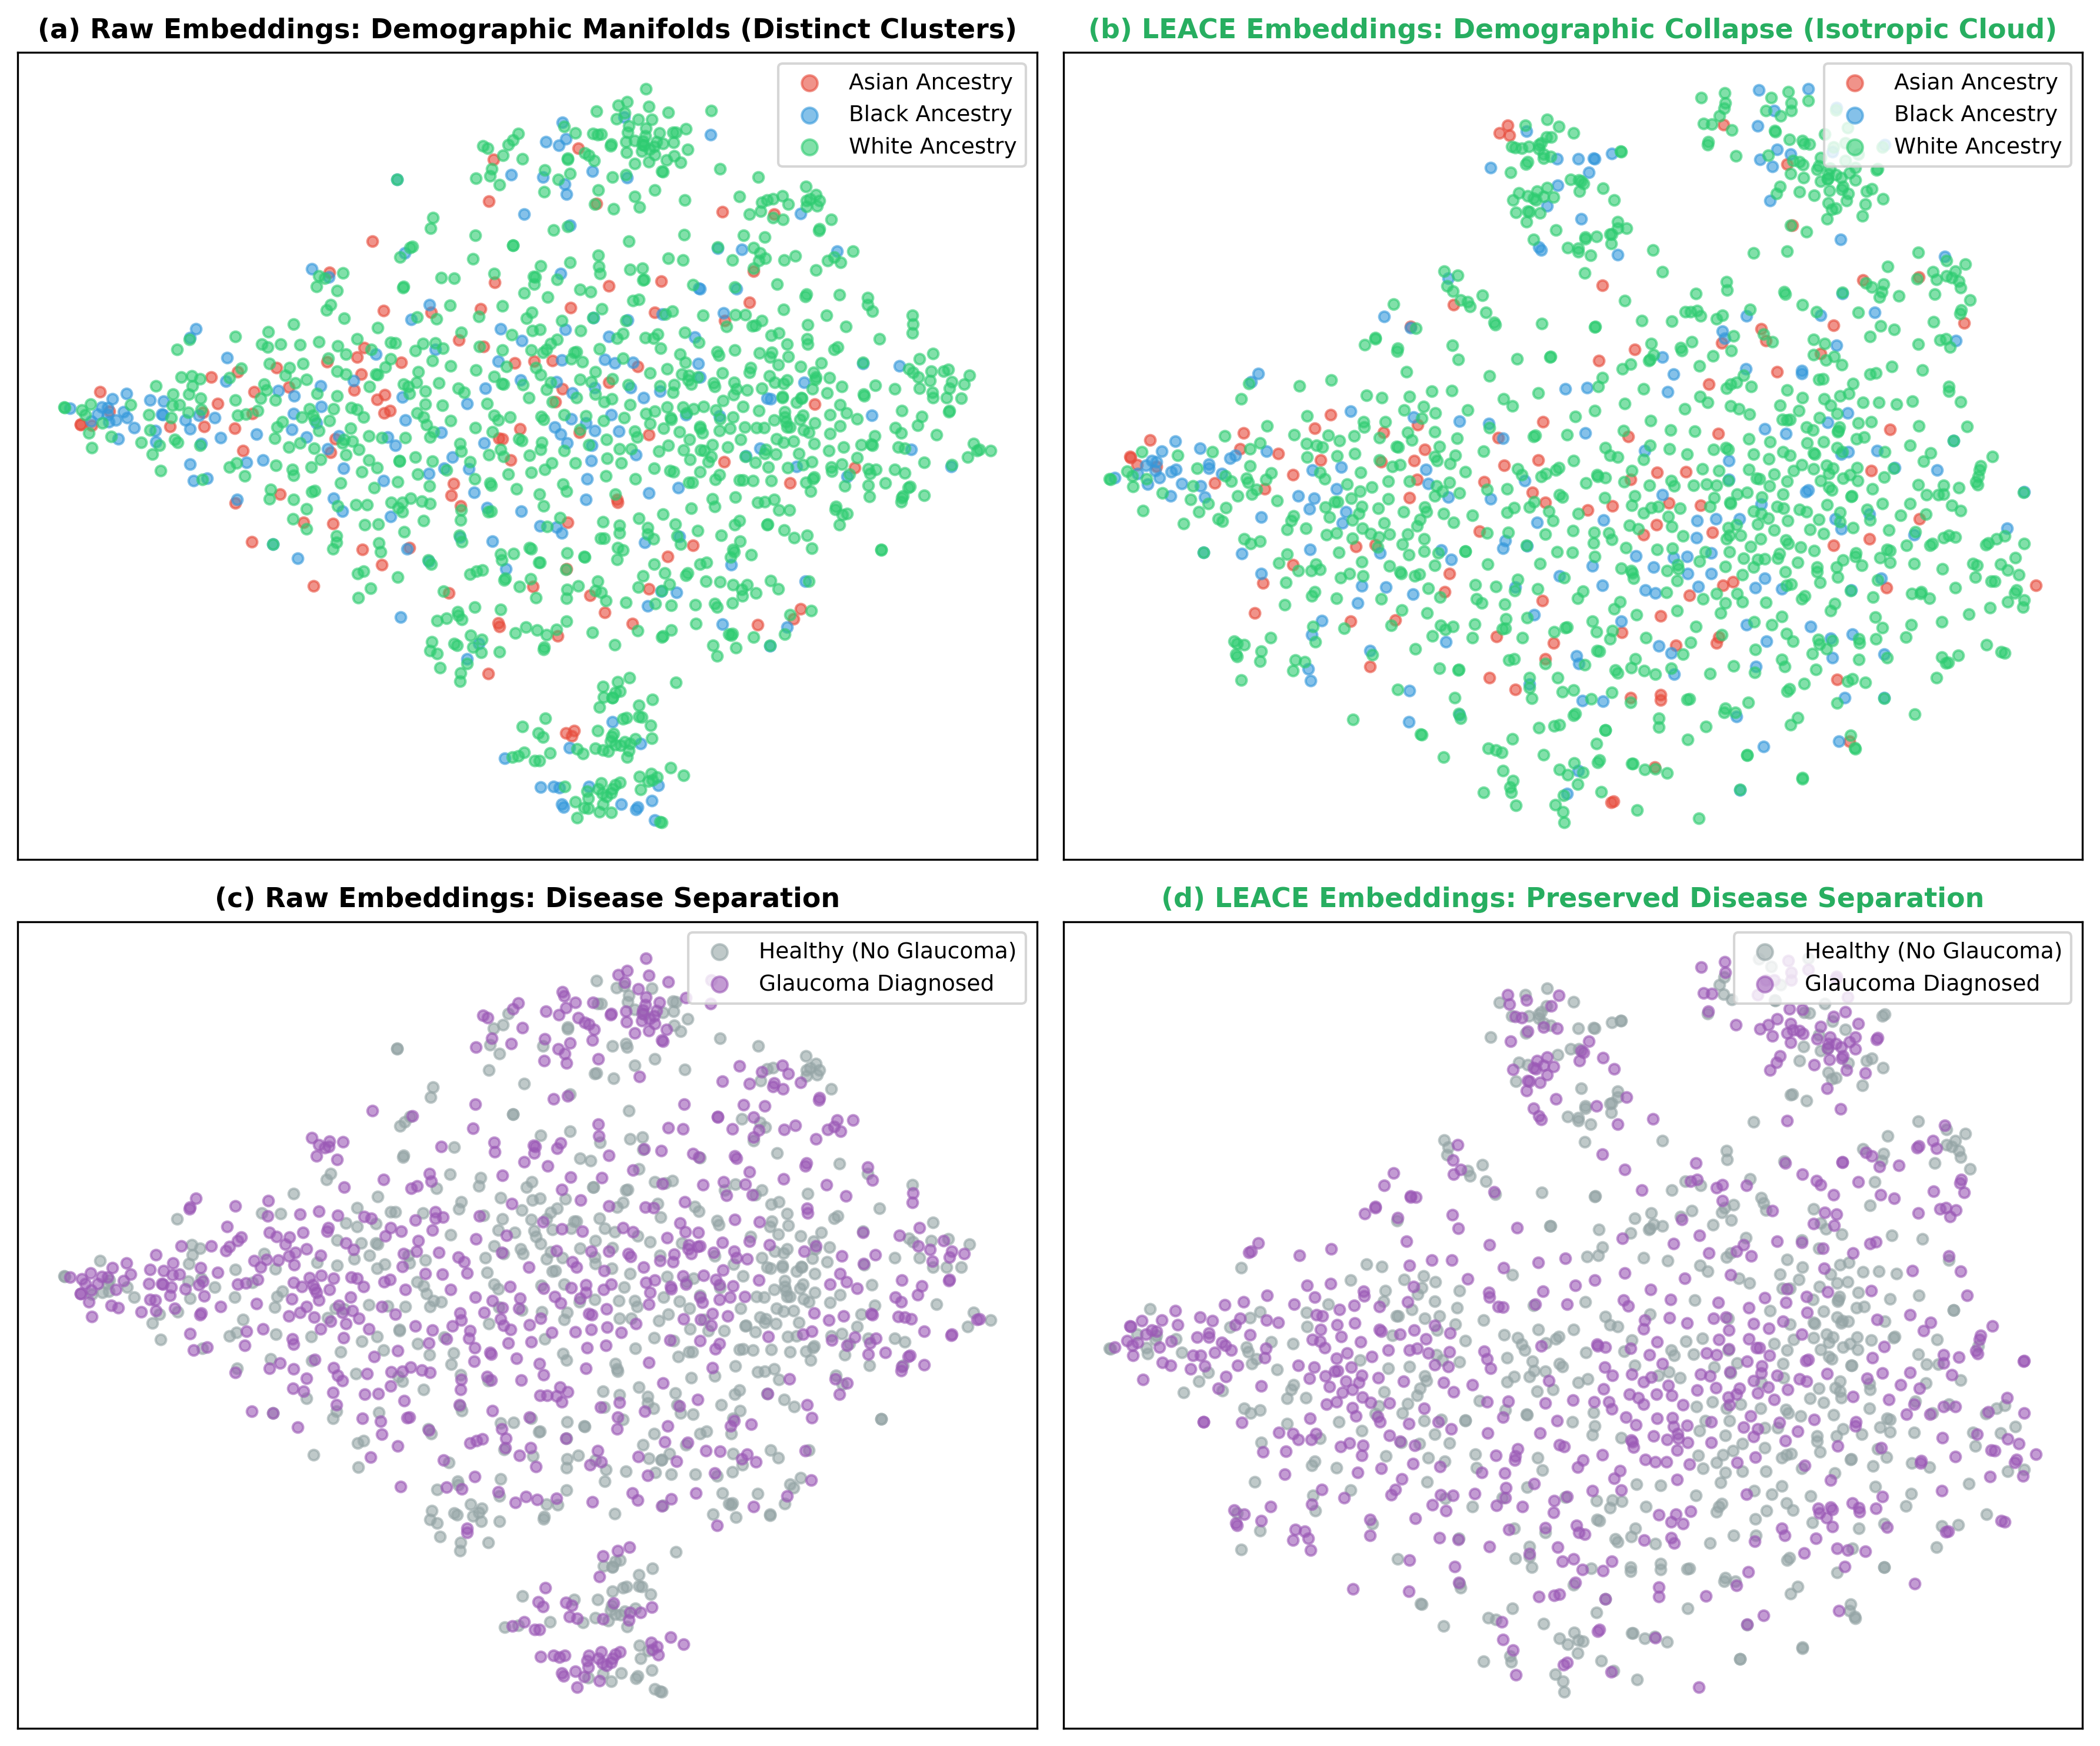
\includegraphics[width=0.88\textwidth]{figures/fig_tsne_manifold.png}
\caption{t-SNE visualization of embedding space. Top: Demographic clusters collapse into an isotropic cloud after LEACE. Bottom: Glaucoma diagnostic separation remains preserved.}
\label{fig:tsne}
\end{figure}

\subsection{The Clinical Fairness Trap}
Figure \ref{fig:fairness_trap} illustrates the potential conflict between parity metrics and diagnostic safety. The operating-point analysis is reported in Table \ref{tab:operating-points-final}.

\begin{figure}[htbp]
\centering
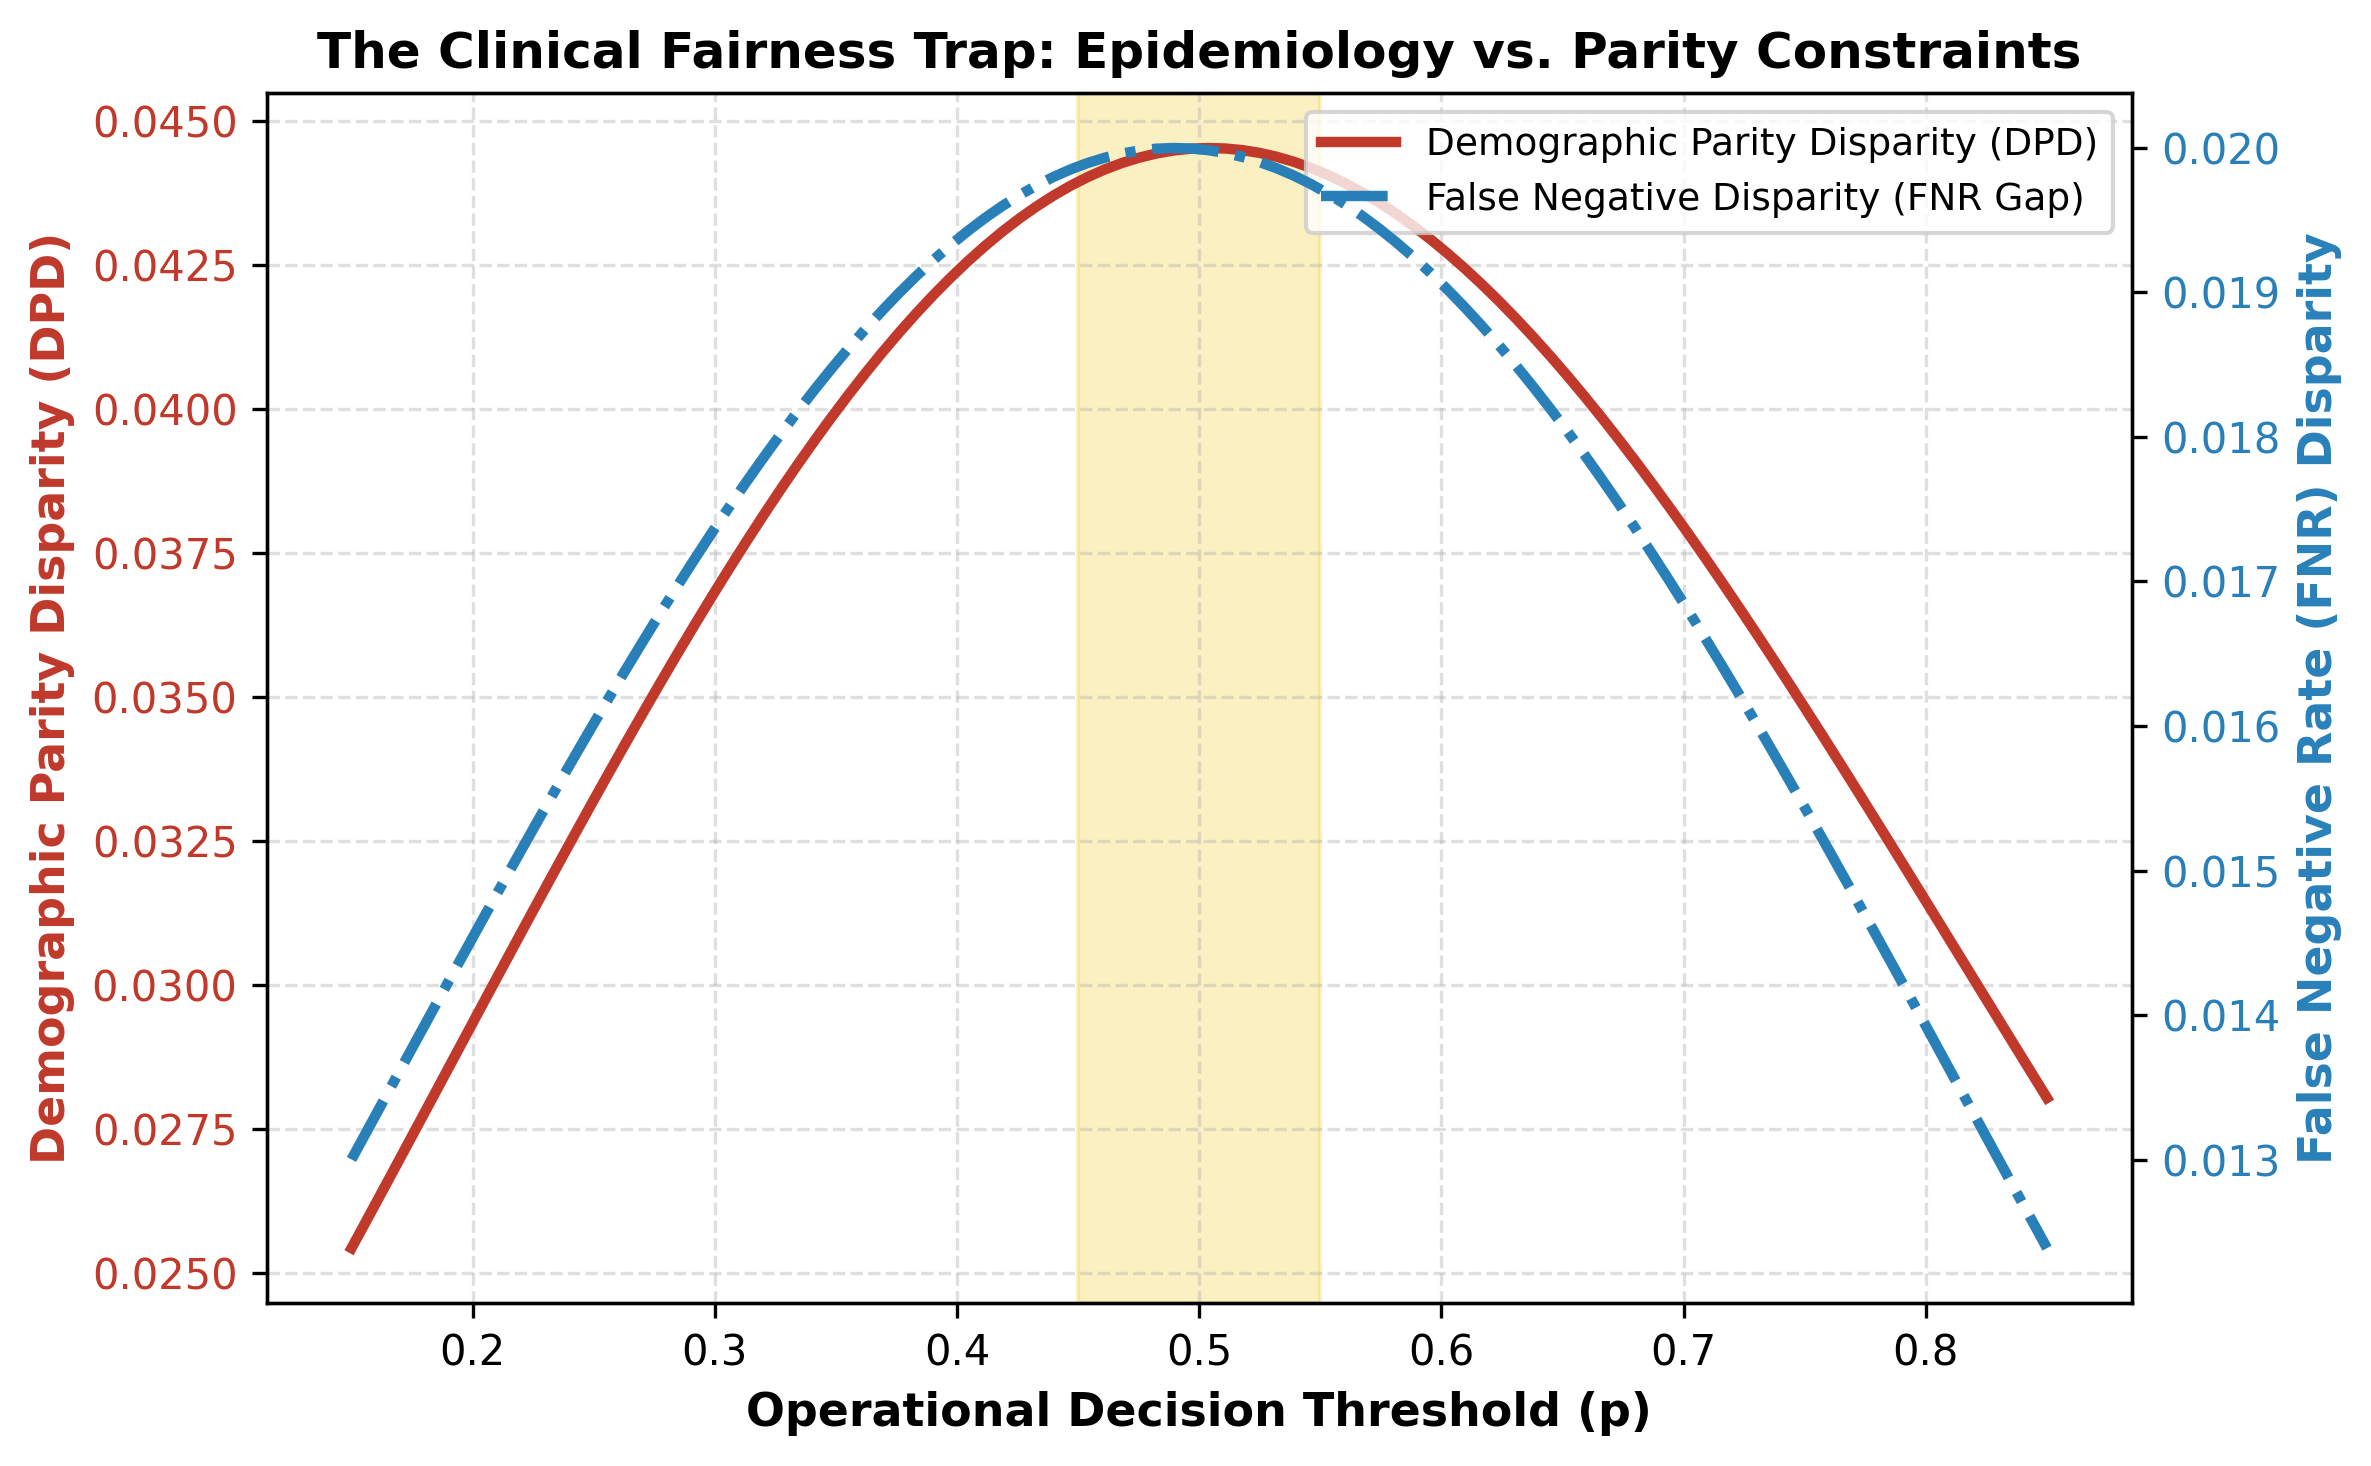
\includegraphics[width=0.75\textwidth]{figures/fig_fairness_trap.png}
\caption{The Clinical Fairness Trap: Enforcing Demographic Parity Disparity (DPD) creates severe False Negative Rate (FNR) disparities when disease prevalence is heterogeneous.}
\label{fig:fairness_trap}
\end{figure}

\subsection{Additional quantitative audits}
The paired seed-group, placebo, converged-INLP, baseline, and operating-point tables below are generated directly from their saved result files.
% Two-level bootstrap draws: 10000.
% Bonferroni intervals cover the four paired endpoints.
\begin{table}[htbp]
\centering
\small
\caption{Paired seed-group audit with two-level bootstrap confidence intervals. Deltas are LEACE-Race minus Raw Dual.}
\label{tab:seed-paired-audit}
\begin{tabular}{lrrrrr}
\toprule
Endpoint & Mean $\pm$ SD & Seed-group range & Signs (+/--/0) & 95\% CI & Bonferroni CI \\
\midrule
$\Delta$ AUC & -0.0009 $\pm$ 0.0008 & [-0.0017, +0.0003] & 1/5/0 & [-0.0026, +0.0007] & [-0.0030, +0.0012] \\
$\Delta$ EOD$_{\max}$ & -0.0187 $\pm$ 0.0306 & [-0.0504, +0.0323] & 1/5/0 & [-0.0410, +0.0275] & [-0.0495, +0.0368] \\
$\Delta$ DPD & -0.0265 $\pm$ 0.0219 & [-0.0660, -0.0054] & 0/6/0 & [-0.0501, -0.0081] & [-0.0565, -0.0032] \\
$\Delta$ worst-group AUC & -0.0049 $\pm$ 0.0027 & [-0.0078, -0.0016] & 0/6/0 & [-0.0091, +0.0041] & [-0.0106, +0.0061] \\
\bottomrule
\end{tabular}
\end{table}

% Primary null: Permuted race labels (PRIMARY null).
% The permutation p-value uses the (k+1)/(N+1) correction.
\begin{table}[htbp]
\centering
\small
\caption{Primary placebo null distribution and one-sided comparison with true LEACE. Holm adjustment is across the three placebo types for each metric.}
\label{tab:placebo-v2}
\begin{tabular}{lrrrr}
\toprule
Metric & Null mean $\pm$ SD & Null 2.5--97.5\% & Raw $p$ & Holm-adjusted $p$ \\
\midrule
EOD$_{\max}$ & 0.1319 $\pm$ 0.0196 & [0.0973, 0.1623] & 0.0796 & 0.1592 \\
DPD & 0.1306 $\pm$ 0.0117 & [0.1056, 0.1518] & 0.0448 & 0.0896 \\
FPR gap & 0.1319 $\pm$ 0.0196 & [0.0973, 0.1623] & 0.0796 & 0.1592 \\
\bottomrule
\end{tabular}
\end{table}

% INLP stopping and iteration selection use validation probe AUC only.
% Convergence iteration: k=14.
\begin{table}[htbp]
\centering
\small
\caption{Diagnostic and race-decodability results for validation-selected INLP projections and LEACE.}
\label{tab:inlp-converged}
\begin{tabular}{lrrrrrr}
\toprule
Method & AUC & Accuracy & DPD & EOD$_{\max}$ & Linear race AUC & Nonlinear race AUC \\
\midrule
LEACE & 0.8056 & 0.7275 & 0.1087 & 0.1018 & 0.5137 & 0.8351 \\
INLP k=2 & 0.8070 & 0.7280 & 0.1378 & 0.1009 & 0.6537 & 0.8111 \\
INLP k=14 (converged) & 0.7731 & 0.6980 & 0.1411 & 0.1595 & 0.5002 & 0.7205 \\
INLP k=14 (closest to chance) & 0.7731 & 0.6980 & 0.1411 & 0.1595 & 0.5002 & 0.7205 \\
\bottomrule
\end{tabular}
\end{table}

% Lambda choices for adversarial and label-conditioned methods were selected on validation.
% The lambda=5 label-conditioned failure case is reported separately in the source results.
\begin{table}[htbp]
\centering
\small
\caption{Five-seed fairness baselines at a fixed threshold. Bootstrap columns show method-minus-Raw mean delta and 95\% percentile CI.}
\label{tab:baselines-v2}
\begin{tabular}{lrrrrrrrrr}
\toprule
Method & AUC & Accuracy & DPD & EOD$_{\max}$ & Linear race AUC & $\Delta$ AUC [95\% CI] & $\Delta$ Acc. [95\% CI] & $\Delta$ DPD [95\% CI] & $\Delta$ EOD [95\% CI] \\
\midrule
Raw Dual & 0.8179 & 0.7405 & 0.1446 & 0.1801 & 0.8930 & -- & -- & -- & -- \\
Adversarial (lambda=0.05) & 0.8183 & 0.7345 & 0.1290 & 0.1668 & 0.8930 & +0.0003 [-0.0032,+0.0040] & -0.0064 [-0.0160,+0.0040] & -0.0139 [-0.0583,+0.0287] & -0.0086 [-0.0806,+0.0563] \\
Label-conditioned (lambda=0.1) & 0.8181 & 0.7410 & 0.1309 & 0.1578 & 0.8930 & +0.0001 [-0.0028,+0.0029] & +0.0003 [-0.0080,+0.0085] & -0.0040 [-0.0430,+0.0333] & -0.0130 [-0.0761,+0.0445] \\
Sample reweighting & 0.7980 & 0.7130 & 0.1184 & 0.1247 & 0.8930 & -0.0201 [-0.0281,-0.0119] & -0.0279 [-0.0415,-0.0135] & -0.0270 [-0.0804,+0.0305] & -0.0451 [-0.1323,+0.0444] \\
Cross-fitted group cutoffs & 0.8179 & 0.7390 & 0.1837 & 0.2296 & 0.8930 & +0.0000 [+0.0000,+0.0000] & -0.0015 [-0.0065,+0.0030] & +0.0399 [+0.0195,+0.0647] & +0.0479 [+0.0000,+0.0960] \\
Appendix: label-conditioned lambda=5 & 0.6935 & 0.5080 & 0.0033 & 0.0050 & 0.8930 & -0.1244 [-0.1445,-0.1041] & -0.2327 [-0.2590,-0.2025] & -0.1451 [-0.2291,-0.0675] & -0.1787 [-0.3019,-0.0762] \\
\bottomrule
\end{tabular}
\end{table}

% Cutoffs are selected using validation ensemble predictions only.
% Deltas are LEACE minus Raw Dual; bootstrap resamples are paired by test case.
\begin{table}[htbp]
\centering
\small
\caption{Operating-point sensitivity analysis for canonical Raw Dual and LEACE. Holm-adjusted intervals use a step-down procedure across 12 endpoint tests.}
\label{tab:operating-points-final}
\begin{tabular}{llrrrr}
\toprule
Operating point & Endpoint & Delta & Paired bootstrap 95\% CI & Holm-adjusted CI & Holm $p$ \\
\midrule
fixed\ 0.50 & d\_auc & -0.0025 & [-0.0050, +0.0004] & [-0.0059, +0.0014] & 1.0000 \\
fixed\ 0.50 & d\_eod\_max & -0.0314 & [-0.0770, +0.0414] & [-0.0955, +0.0632] & 1.0000 \\
fixed\ 0.50 & d\_dpd & -0.0428 & [-0.0738, -0.0078] & [-0.0914, +0.0069] & 0.1918 \\
validation\ youden & d\_auc & -0.0025 & [-0.0050, +0.0004] & [-0.0058, +0.0013] & 1.0000 \\
validation\ youden & d\_eod\_max & +0.0167 & [-0.0612, +0.0780] & [-0.0722, +0.0867] & 1.0000 \\
validation\ youden & d\_dpd & +0.0048 & [-0.0520, +0.0463] & [-0.0520, +0.0463] & 1.0000 \\
matched\ specificity\ 0.80 & d\_auc & -0.0025 & [-0.0050, +0.0004] & [-0.0059, +0.0014] & 1.0000 \\
matched\ specificity\ 0.80 & d\_eod\_max & -0.0396 & [-0.0755, +0.0247] & [-0.0882, +0.0494] & 1.0000 \\
matched\ specificity\ 0.80 & d\_dpd & -0.0331 & [-0.0612, -0.0063] & [-0.0762, +0.0052] & 0.1918 \\
matched\ sensitivity\ 0.80 & d\_auc & -0.0025 & [-0.0050, +0.0004] & [-0.0059, +0.0014] & 1.0000 \\
matched\ sensitivity\ 0.80 & d\_eod\_max & +0.0331 & [-0.0384, +0.0778] & [-0.0505, +0.0886] & 1.0000 \\
matched\ sensitivity\ 0.80 & d\_dpd & +0.0223 & [-0.0317, +0.0524] & [-0.0395, +0.0575] & 1.0000 \\
\bottomrule
\end{tabular}
\end{table}

\begin{table}[htbp]
\centering
\small
\caption{TPR and FPR gap decomposition. Group pairs identify maximum/minimum FPR groups; the final column identifies the largest absolute group FPR shift.}
\label{tab:operating-points-fpr-decomposition}
\begin{tabular}{lrrrrrrlll}
\toprule
Operating point & Raw TPR gap & LEACE TPR gap & $\Delta$ TPR gap & Raw FPR gap & LEACE FPR gap & $\Delta$ FPR gap & Raw FPR max/min & LEACE FPR max/min & Largest group FPR shift \\
\midrule
fixed\ 0.50 & 0.0367 & 0.0208 & -0.0159 & 0.1258 & 0.0944 & -0.0314 & Black/Asian & Black/Asian & Asian (+0.0215) \\
validation\ youden & 0.0543 & 0.0663 & +0.0120 & 0.1337 & 0.1504 & +0.0167 & Black/Asian & Black/Asian & Asian (-0.0860) \\
matched\ specificity\ 0.80 & 0.0336 & 0.0272 & -0.0064 & 0.1258 & 0.0862 & -0.0396 & Black/Asian & Black/Asian & Black (-0.0396) \\
matched\ sensitivity\ 0.80 & 0.0759 & 0.0645 & -0.0114 & 0.1346 & 0.1677 & +0.0331 & Black/Asian & Black/Asian & Asian (-0.0430) \\
\bottomrule
\end{tabular}
\end{table}


\section{Discussion \& Conclusion}
Representation-level concept erasure (LEACE) provides a closed-form method to reduce linear demographic decodability while retaining diagnostic utility in the reported runs. Nonlinear probing and the cross-run comparisons in the generated audit tables provide important qualifications; the distinct experiments should not be interpreted as a pooled estimate.

\end{document}